%%%%%%%%%%%%%%%%%%%%%%%%%%%%%%%%%%%%%%%%%%%%%%%%%%%%%%%%%%%%%%%%%%%%%%%%%%%

\documentclass{standalone}

\usepackage{amsmath}
\usepackage{mathptmx}
\usepackage{pgfplots}
\usetikzlibrary{external}
\tikzexternalize{e-1200-balance}
\pgfplotsset{compat=1.16}

%% IEEE uses Times Roman font, so we'll default to Times.
%% These three commands make up the entire times.sty package.
\renewcommand{\rmdefault}{ptm}
\renewcommand{\ttdefault}{pcr}
\normalfont\selectfont

\begin{document}

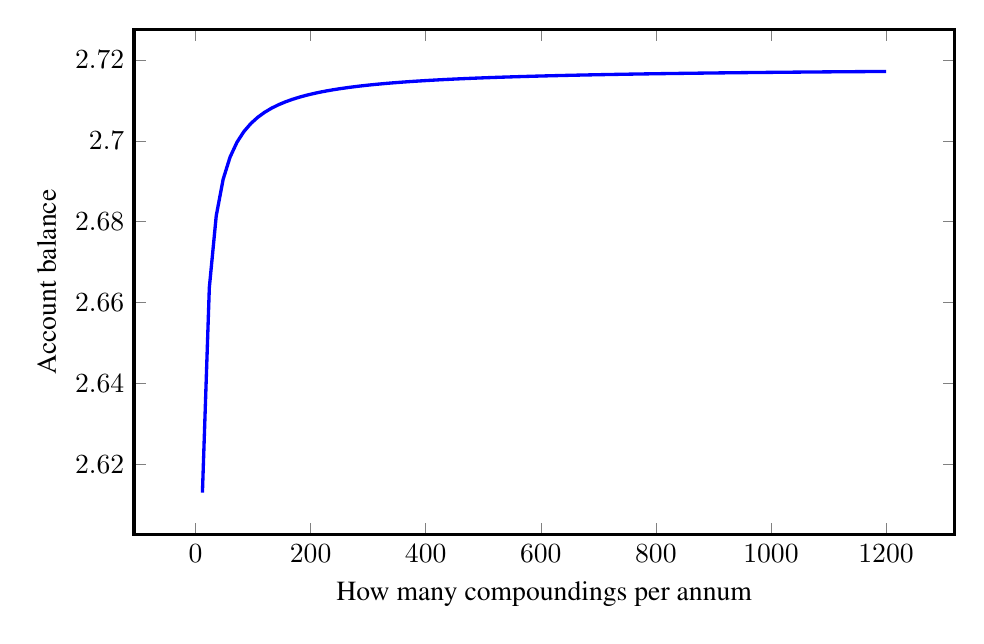
\begin{tikzpicture}
\tikzset{%%
  every mark/.append style={scale=1.0},%%
  scale=1.0%%
}
\pgfplotsset{%%
  every axis/.append style={font=\normalsize}%%
}
%%
\begin{axis}[%%
  axis line style=very thick,%%
  dotStyle/.style={very thick,blue,mark=none},%%
  enlargelimits=true,%%
  height=8cm,%%
  width=12cm,%%
  %% x axis
  xlabel={\normalsize How many compoundings per annum},%%
  xtick={0,200,400,600,800,1000,1200},%%
  xticklabels={$0$,$200$,$400$,$600$,$800$,$1000$,$1200$},%%
  %% y axis
  ylabel={\normalsize Account balance}%%
]
%%
%%
\addplot[dotStyle] coordinates {
  (12, 2.61303529022468)
  (24, 2.6637312580686)
  (36, 2.68146442030086)
  (48, 2.69049659862893)
  (60, 2.69597013933022)
  (72, 2.69964205912664)
  (84, 2.70227616610547)
  (96, 2.70425796641913)
  (108, 2.7058030687704)
  (120, 2.70704149086224)
  (132, 2.70805629671112)
  (144, 2.70890303718626)
  (156, 2.70962027028683)
  (168, 2.71023559714526)
  (180, 2.71076929583941)
  (192, 2.71123659898865)
  (204, 2.71164917108294)
  (216, 2.71201609544627)
  (228, 2.71234455077441)
  (240, 2.71264028548199)
  (252, 2.71290795701252)
  (264, 2.71315137892965)
  (276, 2.71337370376203)
  (288, 2.71357756028318)
  (300, 2.71376515794278)
  (312, 2.71393836727051)
  (324, 2.71409878246196)
  (336, 2.71424777058949)
  (348, 2.71438651065896)
  (360, 2.71451602487468)
  (372, 2.7146372038673)
  (384, 2.71475082720395)
  (396, 2.71485758017661)
  (408, 2.71495806763545)
  (420, 2.71505282545554)
  (432, 2.71514233009615)
  (444, 2.71522700661338)
  (456, 2.71530723541041)
  (468, 2.71538335795098)
  (480, 2.71545568161778)
  (492, 2.71552448385984)
  (504, 2.71559001575164)
  (516, 2.7156525050523)
  (528, 2.71571215885193)
  (540, 2.71576916586335)
  (552, 2.71582369841749)
  (564, 2.71587591420222)
  (576, 2.71592595778548)
  (588, 2.71597396195215)
  (600, 2.71602004888065)
  (612, 2.71606433118108)
  (624, 2.71610691281402)
  (636, 2.71614788990501)
  (648, 2.71618735146945)
  (660, 2.71622538005799)
  (672, 2.71626205233264)
  (684, 2.71629743958228)
  (696, 2.71633160818663)
  (708, 2.71636462003102)
  (720, 2.71639653287921)
  (732, 2.7164274007132)
  (744, 2.71645727403574)
  (756, 2.71648620014698)
  (768, 2.7165142233945)
  (780, 2.71654138540067)
  (792, 2.71656772526711)
  (804, 2.71659327976406)
  (816, 2.71661808350139)
  (828, 2.71664216908483)
  (840, 2.71666556725875)
  (852, 2.7166883070374)
  (864, 2.71671041582513)
  (876, 2.71673191952561)
  (888, 2.71675284264423)
  (900, 2.71677320838041)
  (912, 2.71679303871466)
  (924, 2.71681235448528)
  (936, 2.71683117546462)
  (948, 2.71684952042339)
  (960, 2.71686740719583)
  (972, 2.71688485273597)
  (984, 2.71690187317045)
  (996, 2.71691848385147)
  (1008, 2.71693469939921)
  (1020, 2.71695053374723)
  (1032, 2.71696600018138)
  (1044, 2.71698111137688)
  (1056, 2.71699587943461)
  (1068, 2.71701031590984)
  (1080, 2.71702443184714)
  (1092, 2.71703823780367)
  (1104, 2.71705174387975)
  (1116, 2.717064959741)
  (1128, 2.71707789464227)
  (1140, 2.71709055744812)
  (1152, 2.71710295665594)
  (1164, 2.71711510041066)
  (1176, 2.71712699652684)
  (1188, 2.71713865250261)
  (1200, 2.71715007553642)
};
\end{axis}
\end{tikzpicture}

\end{document}
